\let\negmedspace\undefined
\let\negthickspace\undefined
\documentclass[journal,12pt,onecolumn]{IEEEtran}
\usepackage{cite}
\usepackage{amsmath,amssymb,amsfonts,amsthm}
\usepackage{algorithmic}
\usepackage[version=4]{mhchem}
\usepackage{graphicx}
\usepackage{textcomp}
\usepackage{xcolor}
\usepackage{amsmath}
\usepackage{txfonts}
\usepackage{listings}
\usepackage{enumitem}
\usepackage{mathtools}
\usepackage{gensymb}
\usepackage{comment}
\usepackage[breaklinks=true]{hyperref}
\usepackage{tkz-euclide} 
\usepackage{gvv}                                        
%\def\inputGnumericTable{}                                 
\usepackage[latin1]{inputenc}     
\usepackage{xparse}
\usepackage{color}
\usepackage{array}                                         
\usepackage{longtable}                                     
\usepackage{calc}                                          
\usepackage{multirow}
\usepackage{multicol}
\usepackage{hhline}                                        
\usepackage{ifthen}                                        
\usepackage{lscape}
\usepackage{tabularx}
\usepackage{array}
\usepackage{float}
\newtheorem{theorem}{Theorem}[section]
\newtheorem{problem}{Problem}
\newtheorem{proposition}{Proposition}[section]
\newtheorem{lemma}{Lemma}[section]
\newtheorem{corollary}[theorem]{Corollary}
\newtheorem{example}{Example}[section]
\newtheorem{definition}[problem]{Definition}
\newcommand{\BEQA}{\begin{eqnarray}}
\newcommand{\EEQA}{\end{eqnarray}}
\newcommand{\define}{\stackrel{\triangle}{=}}
\theoremstyle{remark}
\newtheorem{rem}{Remark}
% Marks the beginning of the document
\begin{document}
\title{gg Gate 2011}
\author{ai25btech11014-Gooty Suhas}
\maketitle

\section*{\textbf{PART A: COMMON TO BOTH GEOLOGY AND GEOPHYSICS CANDIDATES}}
\vspace{0.5cm}


\begin{enumerate}
\item The increase in the length of a day on the earth at a rate of 2.4 milliseconds/100 years is due to
\begin{multicols}{2}
\begin{enumerate}
\item prolate tidal bulge  
\item tidal friction  
\item spring tide  
\item bodily earth tide  
\end{enumerate}
\end{multicols}

\item Which of the following rocks contributes the highest amount of radioactive heat in the earth's crust?
\begin{multicols}{4}
\begin{enumerate}
\item basalt  
\item gabbro  
\item dunite  
\item granite  
\end{enumerate}
\end{multicols}

\item The P-wave velocity of the earth's mantle at the Mohorovi\v{c}i\'c discontinuity is
\begin{multicols}{4}
\begin{enumerate}
\item 5.5 km/s  
\item 6.0 km/s  
\item 7.0 km/s  
\item 8.0 km/s  
\end{enumerate}
\end{multicols}


\item Variation of the geomagnetic field observed over the last 500 years indicates that the dipole moment of earth's magnetic field has been
\begin{multicols}{2}
\begin{enumerate}
\item decreasing  
\item increasing  
\item constant  
\item fluctuating randomly  
\end{enumerate}
\end{multicols}

\item Which of the following statements is \textbf{TRUE} for the temperature variation with altitude in the earth's atmosphere?
\begin{enumerate}
\item Temperature increases in both stratosphere and mesosphere  
\item Temperature decreases in stratosphere and increases in mesosphere  
\item Temperature increases in stratosphere and decreases in mesosphere  
\item Temperature decreases in both stratosphere and mesosphere  
\end{enumerate}

\item The deflection of ocean currents in the northern and southern hemispheres is due to
\begin{multicols}{2}
\begin{enumerate}
\item thermohaline circulation  
\item Coriolis effect  
\item El Nino effect  
\item monsoon effect  
\end{enumerate}
\end{multicols}

\item Tsunamis are
\begin{multicols}{2}
\begin{enumerate}
\item gravity waves  
\item acoustic waves  
\item capillary waves  
\item internal waves  
\end{enumerate}
\end{multicols}

\item The planet which contributes maximum to the angular momentum of the solar system is
\begin{multicols}{4}
\begin{enumerate}
\item Earth  
\item Mars  
\item Jupiter  
\item Saturn  
\end{enumerate}
\end{multicols}

\item The depositional feature that forms where a stream emerges from a mountainous region onto a plain is called
\begin{multicols}{2}
\begin{enumerate}
\item alluvial fan  
\item natural levee  
\item delta  
\item point bar  
\end{enumerate}
\end{multicols}

\item Hanging valleys are formed by the geological action of
\begin{multicols}{4}
\begin{enumerate}
\item river  
\item glacier  
\item ocean  
\item wind  
\end{enumerate}
\end{multicols}

\item The surface of discontinuity between older folded sedimentary strata and younger horizontal strata is known as
\begin{multicols}{2}
\begin{enumerate}
\item disconformity  
\item parallel unconformity  
\item angular unconformity  
\item nonconformity  
\end{enumerate}
\end{multicols}

\item The hardest oxide mineral in the Mohs' scale of hardness is
\begin{multicols}{4}
\begin{enumerate}
\item corundum  
\item topaz  
\item quartz  
\item diamond  
\end{enumerate}
\end{multicols}

\item The dominant constituent of ultramafic rocks in the earth's mantle is
\begin{multicols}{2}
\begin{enumerate}
\item orthoclase  
\item olivine  
\item plagioclase  
\item biotite  
\end{enumerate}
\end{multicols}

\item A highly vesicular rock formed by solidification of viscous lava is
\begin{multicols}{4}
\begin{enumerate}
\item tuff  
\item obsidian  
\item volcanic breccia  
\item pumice  
\end{enumerate}
\end{multicols}

\item The most suitable radioactive method for dating Holocene events is
\begin{multicols}{4}
\begin{enumerate}
\item U-Pb  
\item Sm-Nd  
\item Rb-Sr  
\item C-14  
\end{enumerate}
\end{multicols}

\end{enumerate}

\begin{enumerate}
\setcounter{enumi}{15}

\item Which of the following stratigraphic units is  \textbf{NOT} of Proterozoic age?
\begin{multicols}{2}
\begin{enumerate}
\item Tipam Group  
\item Bhima Group  
\item Nallamalai Group  
\item Semri Group  
\end{enumerate}
\end{multicols}

\item Rampura-Agucha in Rajasthan is known for the ore deposit of
\begin{multicols}{4}
\begin{enumerate}
\item gold  
\item tungsten  
\item zinc  
\item iron  
\end{enumerate}
\end{multicols}

\item The geological age of the major hydrocarbon reservoir in the Bombay High oil field is
\begin{multicols}{4}
\begin{enumerate}
\item Cretaceous  
\item Holocene  
\item Oligocene  
\item Miocene  
\end{enumerate}
\end{multicols}

\item The geophysical method for the exploration of disseminated sulfide deposits is
\begin{multicols}{2}
\begin{enumerate}
\item induced polarization  
\item self-potential  
\item gravity  
\item magnetic  
\end{enumerate}
\end{multicols}

\item In a borehole, high pressure gas zone is identified by
\begin{multicols}{2}
\begin{enumerate}
\item sonic logging  
\item resistivity logging  
\item temperature logging  
\item density logging  
\end{enumerate}
\end{multicols}

\item The acceleration due to gravity (g) and universal gravitational constant (G) are related by the expression (Me and Re are the mass and radius of the earth, respectively)
\begin{multicols}{2}
\begin{enumerate}
\item \( g = \frac{GM_e}{R^2} \)  
\item \( g = \frac{GM_e}{R} \)  
\item \( g = \frac{G R_e M_e}{R_a} \)  
\item \( g = \frac{G R_e M^2}{R^2} \)  
\end{enumerate}
\end{multicols}

\item The metamorphic facies diagnostic of subduction zone is
\begin{multicols}{4}
\begin{enumerate}
\item hornblende hornfels  
\item pyroxene hornfels  
\item blueschist  
\item granulite  
\end{enumerate}
\end{multicols}

\item In a formation, if the density increases and elastic constants remain unchanged, then
\begin{enumerate}
\item both P and S wave velocities increase  
\item P wave velocity increases and S wave velocity decreases  
\item both P and S wave velocities decrease  
\item P wave velocity decreases and S wave velocity increases  
\end{enumerate}

\item The Poisson ratio (\( \sigma \)) for rocks in terms of Lame's constants \( \lambda \) and \( \mu \) is
\begin{multicols}{4}
\begin{enumerate}
\item \( \sigma = \frac{\lambda}{2(\lambda + \mu)} \)  
\item \( \sigma = \frac{2\lambda}{2\lambda + \mu} \)  
\item \( \sigma = \frac{\mu}{2(\lambda + \mu)} \)  
\item \( \sigma = \frac{2\mu}{2\lambda + \mu} \)  
\end{enumerate}
\end{multicols}

\item In seismic exploration, 'ground roll' represents
\begin{multicols}{4}
\begin{enumerate}
\item direct wave  
\item surface wave  
\item Stonely wave  
\item shear wave  
\end{enumerate}
\end{multicols}
\newpage
\section*{\textbf{PART B (SECTION 1): FOR GEOLOGY CANDIDATES ONLY}}
\vspace{0.5cm}


\item Choose the correct set of crystal faces for which 'c' crystallographic axis is the zone axis.
\begin{multicols}{2}
\begin{enumerate}
\item (100), (001), (100)  
\item (010), (001), (010)  
\item (010), (110), (100)  
\item (110), (001), (110)  
\end{enumerate}
\end{multicols}

\item The twin plane in the Manebach law is
\begin{multicols}{4}
\begin{enumerate}
\item (010)  
\item (001)  
\item (100)  
\item (021)  
\end{enumerate}
\end{multicols}

\item The optic sign of a mineral showing increase (i) and decrease (d) in interference colors after insertion of mica plate is

\begin{figure}[H]
    \centering
    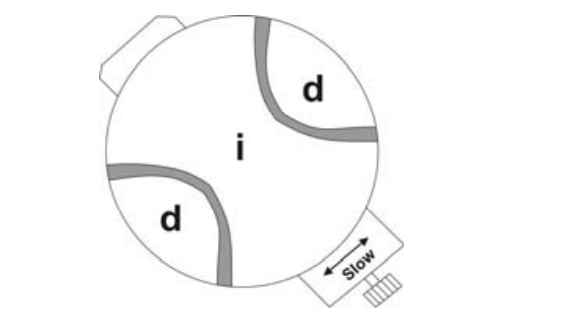
\includegraphics[width=0.4\textwidth]{figs/fig1.png}
    \caption{Image for questions 28}
    \label{fig:question28}
\end{figure}


\begin{multicols}{2}
\begin{enumerate}
\item uniaxial positive  
\item uniaxial negative  
\item biaxial positive  
\item biaxial negative  
\end{enumerate}
\end{multicols}

\item The igneous rock falling in the shaded field of the diagram is

\begin{figure}[H]
    \centering
    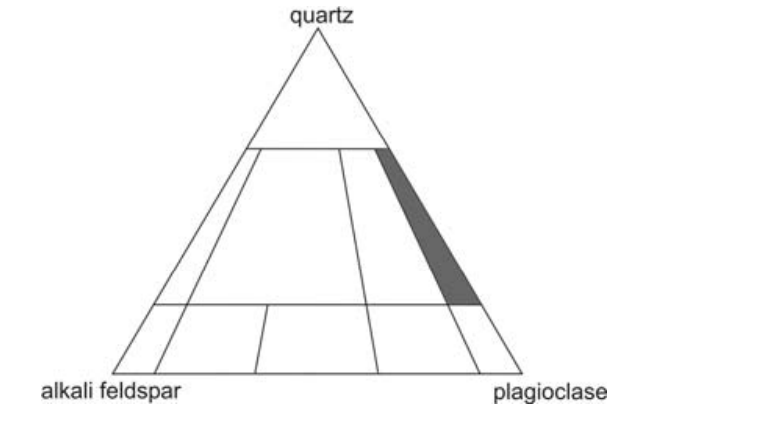
\includegraphics[width=0.4\textwidth]{figs/fig2.png}
    \caption{Image for questions 29}
    \label{fig:question29}
\end{figure}




\begin{multicols}{4}
\begin{enumerate}
\item granite  
\item syenite  
\item tonalite  
\item monzonite  
\end{enumerate}
\end{multicols}

\item The figure below is the photomicrograph of a chloritoid mica schist in which chloritoid forms porphyroblasts. The formation of porphyroblasts in the crenulated matrix is 


\begin{figure}[H]
    \centering
    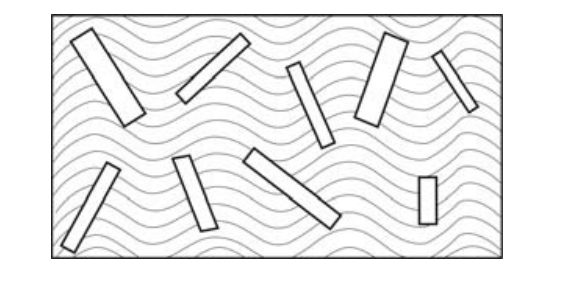
\includegraphics[width=0.4\textwidth]{figs/fig3.png}
    \caption{Image for questions 30}
    \label{fig:question30B}
\end{figure}







\begin{multicols}{2}
\begin{enumerate}
\item pre-tectonic  
\item early syn-tectonic  
\item late syn-tectonic  
\item post-tectonic  
\end{enumerate}
\end{multicols}
\end{enumerate}

\begin{enumerate}
\setcounter{enumi}{30}

\item A pelitic rock is uplifted after high pressure metamorphism in the earth's crust. The mineral transformation due to uplift will be
\begin{multicols}{2}
\begin{enumerate}
\item kyanite to sillimanite  
\item sillimanite to kyanite  
\item andalusite to kyanite  
\item andalusite to sillimanite  
\end{enumerate}
\end{multicols}

\item Which of the following sedimentary structures is  \textbf{NOT} a 'tool mark'?
\begin{multicols}{4}
\begin{enumerate}
\item prod cast  
\item groove cast  
\item flute cast  
\item bounce cast  
\end{enumerate}
\end{multicols}






\item The echinoids transformed from epifaunal to infaunal type in the Jurassic times. Consider the following morphological changes:

\begin{flushleft}
\textbf{P} increase in size of spines  \\
\textbf{Q} increase in number of spines  \\
\textbf{R} development of phyllodes  \\
\textbf{S} bulging of shell
\end{flushleft}

Which of the above changes were functionally advantageous in this transformation?

\begin{multicols}{4}
\begin{enumerate}
\item P, Q, R, S  
\item P, S only  
\item Q, S only  
\item Q, R only  
\end{enumerate}
\end{multicols}





\newpage



\item Match the Bivalvia in Group I with the corresponding ecology in Group II.

\begin{multicols}{2}
\textbf{Group I}  
\begin{flushleft}
P. Mytilus\\
Q. Pecten\\
R. Ostrea\\
S. Mya
\end{flushleft}

\columnbreak

\textbf{Group II}  
\begin{flushleft}
1. Cemented\\
2. Swimmer\\
3. Bysally attached\\
4. Infaunal\\
5. Floating
\end{flushleft}
\end{multicols}

\begin{multicols}{2}
\begin{enumerate}
\item P--1, Q--2, R--3, S--5  
\item P--3, Q--2, R--1, S--4  
\item P--2, Q--3, R--5, S--1  
\item P--2, Q--4, R--5, S--3  
\end{enumerate}
\end{multicols}




\item Determine the correctness or otherwise of the following statements:

\textbf{Assertion (a):} The Lower Gondwana rocks in Central India, containing brachiopod genera Productus, Spiriferina and Reticularia, are considered to have formed by transgression of the Tethys Sea in Peninsular India during Permian.

\textbf{Reason (r):} The brachiopods are marine organisms and the stratigraphic ranges of the brachiopod species of the formation suggest Permian age.

\begin{enumerate}
\item Both (a) and (r) are true and (r) is the correct reason for (a)  
\item (a) is true but (r) is false  
\item (a) is false but (r) is true  
\item Both (a) and (r) are true but (r) is not the correct reason for (a)  
\end{enumerate}

\item In the following lithostratigraphic units, which of the formations are of Palaeocene and/or Eocene age?

\begin{flushleft}
\textbf{P} Barail Formation \\
\textbf{Q} Subathu Formation \\
\textbf{R} Sylhet Limestone \\
\textbf{S} Kamlial Formation
\end{flushleft}

\begin{multicols}{4}
\begin{enumerate}
\item P, Q  
\item Q, R  
\item R, S  
\item P, S  
\end{enumerate}
\end{multicols}



\item The microfaunal assemblages in a fining upward stratigraphic sequence are given below:

\textbf{Top:} High abundance of \textit{Globigerina, Globorotalia} and \textit{Orbulina}

\textbf{Middle:} Moderate abundance of \textit{Uvigerina, Cassidulina} and low abundance of \textit{Globigerina}

\textbf{Bottom:} Moderate abundance of \textit{Ammonia, Elphidium} and \textit{Quinqueloculina}
The sequence corresponds to
\begin{multicols}{4}
\begin{enumerate}
\item lowstand systems tract  
\item highstand systems tract  
\item transgressive systems tract  
\item shelf margin systems tract  
\end{enumerate}
\end{multicols}






\item Match the geomorphological features in Group I with the corresponding characteristics in Group II.

\begin{multicols}{2}
\textbf{Group I}  
\begin{flushleft}
P. Atolls\\
Q. Mesa\\
R. Barchans
\end{flushleft}

\columnbreak

\textbf{Group II}  
\begin{flushleft}
1. reefs parallel to the shore and separated by deep lagoon\\
2. broad flat topped hill capped by resistant rock and bounded by cliffs\\
3. circular reefs that rim lagoons\\
4. crescent shaped sand dunes
\end{flushleft}
\end{multicols}

\begin{multicols}{4}
\begin{enumerate}
\item P--1, Q--2, R--3  
\item P--3, Q--2, R--4  
\item P--3, Q--4, R--1  
\item P--2, Q--4, R--1  
\end{enumerate}
\end{multicols}











\item Match the optical properties in Group I with the corresponding mineral in Group II.

\begin{multicols}{2}
\textbf{Group I}  
\begin{flushleft}
1. internal reflections\\
2. bireflectance\\
3. triangular pits\\
4. pyrrhotite
\end{flushleft}

\columnbreak

\textbf{Group II}  
\begin{flushleft}
P. galena\\
Q. sphalerite\\
R. magnetite\\
S. pyrrhotite
\end{flushleft}
\end{multicols}

\begin{multicols}{4}
\begin{enumerate}
\item P--4, Q--3, R--1  
\item P--3, Q--2, R--4  
\item P--2, Q--4, R--1  
\item P--2, Q--1, R--4  
\end{enumerate}
\end{multicols}






\item Which of the following bands (in micrometre) is \textbf{NOT} suitable for earth observation in satellite remote sensing?
\begin{multicols}{4}
\begin{enumerate}
\item 0.30--0.35  
\item 0.53--0.58  
\item 0.62--0.67  
\item 0.74--0.78  
\end{enumerate}
\end{multicols}

\end{enumerate}


\begin{enumerate}[resume]

\item Thermal maturation of hydrocarbon source rocks can be determined from
\begin{enumerate}
\item temperature of the borehole drilled into the source rock  
\item \(^{18}O/^{16}O\) ratio of the source rock  
\item Mg/Ca ratio of foraminifera in the source rock  
\item color of spores and pollens in the source rock  
\end{enumerate}

\item Determine the correctness or otherwise of the following statements:

\textbf{Assertion (a)} Strontium concentration in a basic magma decreases with fractional crystallization of plagioclase.

\textbf{Reason (r)} Strontium is a compatible trace element in plagioclase during magmatic crystallization.

\begin{enumerate}
\item Both (a) and (r) are true and (r) is the correct reason for (a)  
\item (a) is true but (r) is false  
\item (a) is false but (r) is true  
\item Both (a) and (r) are true but (r) is not the correct reason for (a)  
\end{enumerate}

\item Which of the following is true for the coordination number \(n\) of aluminium?
\begin{enumerate}
\item \(n = 4\) in both plagioclase and garnet  
\item \(n = 6\) in both plagioclase and garnet  
\item \(n = 4\) in plagioclase and \(n = 6\) in garnet  
\item \(n = 6\) in plagioclase and \(n = 4\) in garnet  
\end{enumerate}

\item If the dissociation constant of pure natural water at 50\(^\circ\)C is \(10^{-13}\), the pH of the water will be
\begin{multicols}{4}
\begin{enumerate}
\item 6.00  
\item 6.55  
\item 7.00  
\item 7.55  
\end{enumerate}
\end{multicols}

\item Choose the correct statement:
\begin{enumerate}
\item Sandstone forms aquifers and sandy shale forms aquifuges  
\item Sandstone forms aquifers and sandy shale forms aquitards  
\item Sandstone forms aquicludes and sandy shale forms aquifuges  
\item Both sandstone and sandy shale form aquifuges  
\end{enumerate}

\item The slow, permanent and continuous deformation of materials under constant load is called
\begin{multicols}{4}
\begin{enumerate}
\item strain hardening  
\item stress stiffening  
\item work hardening  
\item creep  
\end{enumerate}
\end{multicols}

\item Which of the following lithostratigraphic units hosts lignite at Neyveli?
\begin{multicols}{2}
\begin{enumerate}
\item Ariyalur Formation  
\item Cuddalore Formation  
\item Kamthi Beds  
\item Pali Beds  
\end{enumerate}
\end{multicols}

\subsection*{Common Data for Questions 48 and 49:}  
\vspace{0.5cm}
The figure below is the schematic geological map of a flat terrane. 
\vspace{0.5cm}
\begin{figure}[H]
    \centering
    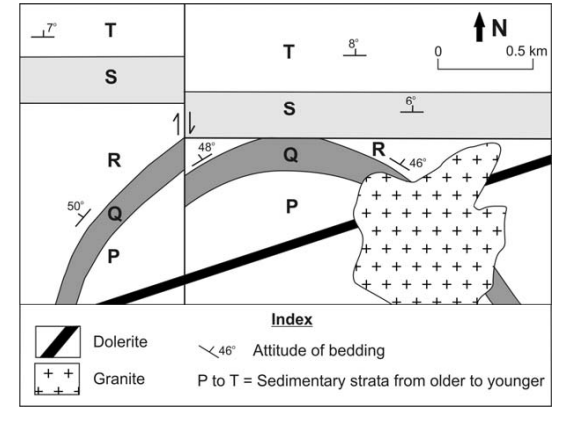
\includegraphics[width=0.6\textwidth]{figs/fig4.png}
    \caption{Image for questions 48,49}
    \label{fig:question48,49}
\end{figure}






\item The strata P, Q and R have been folded into a
\begin{multicols}{2}
\begin{enumerate}
\item north-plunging anticlinal antiform  
\item south-plunging anticlinal antiform  
\item north-plunging synclinal antiform  
\item south-plunging synclinal antiform  
\end{enumerate}
\end{multicols}

\item The granite pluton intruded
\begin{enumerate}
\item before folding and faulting  
\item before faulting but after folding  
\item after development of unconformity but before faulting  
\item after development of unconformity and faulting  
\end{enumerate}

\subsection*{Common Data for Questions 50 and 51: }  
\vspace{0.5cm}
Oceanic crust is generally covered by sediments. In a convergent tectonic setting, basaltic crust, along with its sedimentary cover, is subducted beneath continental plate. In such a setting, magmatism leads to the
formation of a continental arc. 
\vspace{0.5cm}











\item The magma series typical of the arc is
\begin{enumerate}
\item alkaline  
\item alkaline-shoshonitic  
\item tholeiitic  
\item calc-alkaline  
\end{enumerate}

\end{enumerate}


\begin{enumerate}
\setcounter{enumi}{50}

\item The type of sulphide mineral deposit formed in this tectonic setting is
\begin{multicols}{2}
\begin{enumerate}
\item Porphyry copper  
\item Mississippi Valley lead and zinc  
\item Besshi copper and zinc  
\item Kuroko copper  
\end{enumerate}
\end{multicols}


\subsection*{Statement for Linked Answer Questions 52 and 53: }  
\vspace{0.5cm}

The modal analysis of a sandstone shows: Quartz 54\%, Mica 3\%, Feldspar 33\%, Cement 5\%, Matrix 5\%
\vspace{0.5cm}


\item The sandstone belongs to the class  
\begin{multicols}{4}
\begin{enumerate}
\item Quartz wacke  
\item Arkosic wacke  
\item Arkose  
\item Quartz arenite  
\end{enumerate}
\end{multicols}

\item In which of the following conditions the correct sandstone class in the previous question might have formed?

\begin{flushleft}
P -- Warm arid climate\\
Q -- Humid tropical climate\\
R -- Long exposure and transportation\\
S -- Quick burial without much transportation
\end{flushleft}

\begin{multicols}{4}
\begin{enumerate}
\item P -- S  
\item P -- R  
\item Q -- R  
\item Q -- S  
\end{enumerate}
\end{multicols}


\subsection*{Statement for Linked Answer Questions 54 and 55: }  
\vspace{0.5cm}

Lithostratigraphic units of different ages and hosting different ore deposits are exposed in Peninsular India
\vspace{0.5cm}







\item Which of the following lithostratigraphic units is of Palaeoproterozoic age?
\begin{multicols}{2}
\begin{enumerate}
\item Aravalli Supergroup  
\item Dharwar Supergroup  
\item Vindhyan Supergroup  
\item Sukma Group  
\end{enumerate}
\end{multicols}

\item The host rock and associated metal deposit found in the correct lithostratigraphic unit in the previous question is
\begin{multicols}{2}
\begin{enumerate}
\item chlorite schist -- copper  
\item dolomite -- lead and zinc  
\item banded haematite quartzite -- iron  
\item chlorite schist -- antimony  
\end{enumerate}
\end{multicols}

\end{enumerate}
\newpage
\section*{\textbf{PART B (SECTION 2): FOR GEOLOGY CANDIDATES ONLY}}
\vspace{0.5cm}

\begin{enumerate}
\setcounter{enumi}{25}










\item Rayleigh number associated with convection in the earth's interior is proportional to the ratio of
\begin{enumerate}
\item buoyancy force to diffusive viscous force  
\item buoyancy force to gravitational force  
\item diffusive viscous force to gravitational force  
\item gravitational force to buoyancy force  
\end{enumerate}

\item Shadow zones for direct P- and S-waves lie between
\begin{enumerate}
  \item 102\textdegree{} to 142\textdegree{} for both direct P- and S-waves  
  \item 102\textdegree{} to 180\textdegree{} for direct P-wave and 102\textdegree{} to 142\textdegree{} for direct S-wave  
  \item 102\textdegree{} to 180\textdegree{} for both direct P- and S-waves  
  \item 102\textdegree{} to 142\textdegree{} for direct P-wave and 102\textdegree{} to 180\textdegree{} for direct S-wave  
\end{enumerate}

\item Snell's law of refraction deals with which of the following properties of refracted waves?
\begin{multicols}{4}
\begin{enumerate}
\item amplitude  
\item direction  
\item energy  
\item phase  
\end{enumerate}
\end{multicols}

\item In seismic reflection, the seismic trace is modeled as
\begin{enumerate}
\item convolution of source wavelet with the reflection coefficient series  
\item multiplication of source wavelet with the reflection coefficient series  
\item correlation of source wavelet with the reflection coefficient series  
\item addition of source wavelet with the reflection coefficient series  
\end{enumerate}

\item From the following figure, choose the correct multiple reflection events encountered in seismic exploration  

\begin{figure}[H]
    \centering
    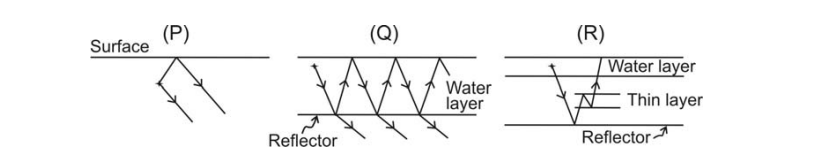
\includegraphics[width=0.8\textwidth]{figs/fig5.png}
    \caption{Image for questions 30}
    \label{fig:question30}
\end{figure}

\begin{enumerate}
\item P is peg leg multiple, Q is ghost, R is long path multiple  
\item P is ghost, Q is simple multiple, R is reverberation  
\item P is peg leg multiple, Q is simple multiple, R is reverberation  
\item P is ghost, Q is reverberation, R is peg leg multiple  
\end{enumerate}

\item Match the items in \textbf{Group I} with those in \textbf{Group II}

\begin{multicols}{2}
\textbf{Group I}  
\begin{flushleft}
P. Correlation in frequency domain\\
Q. Phase spectrum\\
R. Frequency interval\\
S. Undersampling
\end{flushleft}

\columnbreak

\textbf{Group II}  
\begin{flushleft}
1. Reciprocal of total signal duration\\
2. Aliasing\\
3. Product of Fourier transform and its conjugate\\
4. Autocorrelation\\
5. Hilbert transform
\end{flushleft}
\end{multicols}

\begin{multicols}{2}
\begin{enumerate}
\item P--3, Q--5, R--1, S--2  
\item P--3, Q--4, R--2, S--1  
\item P--3, Q--4, R--1, S--2  
\item P--2, Q--3, R--4, S--5  
\end{enumerate}
\end{multicols}


\item The derivative of the following boxcar function is

\begin{figure}[H]
    \centering
    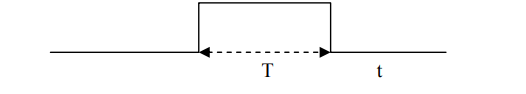
\includegraphics[width=0.8\textwidth]{figs/fig6.png}
    \caption{Image for questions 33}
    \label{fig:question32}
\end{figure}

\begin{enumerate}
\begin{multicols}{2}
\item  \begin{figure}[H]
    \centering
    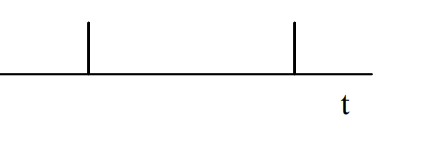
\includegraphics[width=0.4\textwidth]{figs/fig7.png}
    \caption{Image for questions 33}
    \label{fig:question32a}
\end{figure}
\item  \begin{figure}[H]
    \centering
    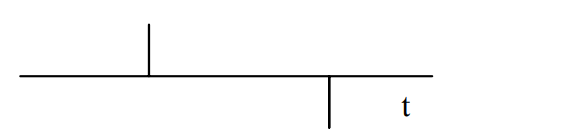
\includegraphics[width=0.4\textwidth]{figs/fig8.png}
    \caption{Image for questions 33}
    \label{fig:question32b}
\end{figure}

\item \begin{figure}[H]
    \centering
    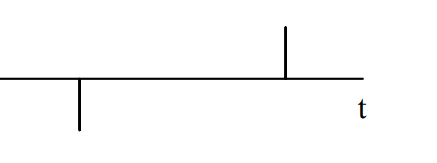
\includegraphics[width=0.4\textwidth]{figs/fig9.png}
    \caption{Image for questions 33}
    \label{fig:question32c}
\end{figure}
 
\item \begin{figure}[H]
    \centering
    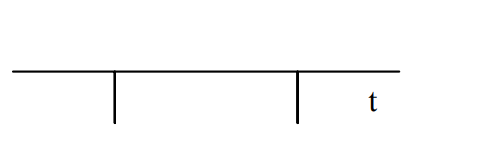
\includegraphics[width=0.4\textwidth]{figs/fig10.png}
    \caption{Image for questions 33}
    \label{fig:question32d}
\end{figure}
\end{multicols}
\end{enumerate}

\item Gravity measurement is made on a ship sailing at the speed of 6 knots in the direction N65\textdegree{}E at 20\textdegree{}N latitude. The Eotvos correction (in mGal) is
\begin{enumerate}
\begin{multicols}{4}
\item +38.5  
\item +24.5  
\item --35.5  
\item --39.5  
\end{multicols}
\end{enumerate}

\end{enumerate}

\begin{enumerate}
\setcounter{enumi}{34}

\item Isostatic residual anomaly over a mountainous terrain is due to  
\begin{enumerate}
\item gravitational effect of compensating mass  
\item long wavelength variations of topography  
\item short wavelength variations of topography  
\item density inhomogeneities in the upper and middle crust  
\end{enumerate}

\end{enumerate}


\begin{enumerate}
\setcounter{enumi}{35}

\item In magnetic data reduction, the altitude correction at magnetic equator is 0.015 nT/m. Altitude correction (in nT/m) at the magnetic poles is  
\begin{multicols}{4}
\begin{enumerate}
\item 0.015  
\item 0.030  
\item 0.045  
\item 0.060  
\end{enumerate}
\end{multicols}

\item The Larmor precession frequency (in Hz) measured by proton precession magnetometer for a total field of 50,000 nT is (gyromagnetic ratio of proton \(Y_p = 0.267513 \, \text{nT}^{-1}\text{s}^{-1}\))  
\begin{multicols}{4}
\begin{enumerate}
\item 1890  
\item 2020  
\item 2130  
\item 2420  
\end{enumerate}
\end{multicols}

\item Gamma ray log measurements are used to quantify  
\begin{enumerate}
\item hydrocarbon saturation  
\item porosity of the formation  
\item density of the formation  
\item volume of shale in the formation  
\end{enumerate}

\item Free fluid index (FFI) of a formation is estimated from  
\begin{multicols}{4}
\begin{enumerate}
\item neutron log  
\item latero log  
\item induction log  
\item NMR log  
\end{enumerate}
\end{multicols}

\item Compton scattering takes place if the energy of gamma rays lies in the range of  
\begin{enumerate}
\item 10 KeV to 50 KeV  
\item 50 KeV to 100 KeV  
\item 100 KeV to 2.0 MeV  
\item 2.0 MeV to 3.5 MeV  
\end{enumerate}

\item Which of the following Maxwell's equations is NOT CORRECT for time varying electromagnetic field?  
\begin{multicols}{2}
\begin{enumerate}
\item \(\nabla \times \vec{E} = \vec{J}\)  
\item \(\nabla \times \vec{E} = -\frac{\partial \vec{B}}{\partial t}\)  
\item \(\nabla \cdot \vec{D} = \rho\)  
\item \(\nabla \cdot \vec{B} = 0\)  
\end{enumerate}
\end{multicols}

\item The apparent resistivity sounding curve representing the resistivity structure \(\rho_1 > \rho_2 < \rho_3 < \rho_4\) is  
\begin{multicols}{2}
\begin{enumerate}
\item HK-type  
\item HA-type  
\item KH-type  
\item KQ-type  
\end{enumerate}
\end{multicols}

\item Forced movement of fluids through porous rocks gives rise to  
\begin{multicols}{2}
\begin{enumerate}
\item streaming potential  
\item Nernst potential  
\item mineralization potential  
\item liquid junction potential  
\end{enumerate}
\end{multicols}






\item Match the EM methods in Group I with the corresponding quantity measured by them in Group II.

\begin{multicols}{2}
\textbf{Group I}  
\begin{flushleft}
P. VLF\\
Q. Two-frame\\
R. Slingram\\
S. TURAM
\end{flushleft}

\columnbreak

\textbf{Group II}  
\begin{flushleft}
1. Amplitude ratio and phase difference\\
2. Real and imaginary components\\
3. Dip angle\\
4. Amplitude ratio
\end{flushleft}
\end{multicols}

\begin{multicols}{2}
\begin{enumerate}
\item P--2, Q--4, R--3, S--1  
\item P--3, Q--4, R--2, S--1  
\item P--3, Q--4, R--1, S--2  
\item P--2, Q--3, R--4, S--1  
\end{enumerate}
\end{multicols}

\end{enumerate}


\begin{enumerate}
\setcounter{enumi}{44}

\item Arrange the following electromagnetic methods in the decreasing order of depth of investigation.  \\
P -- Time domain EM method  \\
Q -- Magnetotelluric method  \\
R -- VLF method  \\
S -- Ground Penetrating Radar method  

\begin{multicols}{2}
\begin{enumerate}
  \item \(P > Q > S > R\)
  \item \(S > Q > P > R\)
  \item \(Q > P > R > S\)
  \item \(Q > R > P > S\)
\end{enumerate}
\end{multicols}


\item The least squares generalized inverse of an overdetermined problem is expressed as  
\begin{multicols}{2}
\begin{enumerate}
\item \((G^T G)^{-1} G^T\)  
\item \((G^T G)^{-1}\)  
\item \(G^T (G G^T)^{-1}\)  
\item \((G G^T)^{-1}\)  
\end{enumerate}
\end{multicols}
\end{enumerate}

\begin{enumerate}[resume]

\item The primary field (\(H_p\)) in EM prospecting is represented by \(H_p = K \sin(\omega t)\). Which is the correct expression for induced e.m.f. (\(e_s\)) in the subsurface conductor? (K and \(K'\) are constants)

\begin{enumerate}
\item \(e_s = K' \sin(\omega t - \phi)\)  
\item \(e_s = K' \cos(\omega t - 2\phi)\)  
\item \(e_s = K' \sin(\omega t - \frac{\phi}{2})\)  
\item \(e_s = K' \cos(\omega t - \phi)\)  
\end{enumerate}


\subsection*{Common Data for Questions 48 and 49:}  
\vspace{0.5cm}
Time series P and Q are given by  
P = \{1, -1, -2, 0, 1\}  
Q = \{1, 0, -1\}
\vspace{0.5cm}

\item The convolution of P and Q is  
\begin{enumerate}
\item \{-1, 0, 3, 1, -3, -1, 1\}  
\item \{1, -1, -3, 1, 3, 0, -1\}  
\item \{1, -1, -3, -1, 3, 1, -1\}  
\item \{1, 0, 3, 1, -3, -1, 1\}  
\end{enumerate}


\item P is similar and most out of phase to Q at a lag of  
\begin{enumerate}
\begin{multicols}{4}

\item 0  
\item 1  
\item 2  
\item 3  
\end{multicols}
\end{enumerate}

\end{enumerate}

\subsection*{Common Data for Questions 50 and 51:}  
\vspace{0.5cm}
An asymmetric split spread extends from \(x_1 = -400\, \text{m}\) to \(x_2 = 800\, \text{m}\). A reflection observed on the spread yields  
\(t_1 = 0.997\, \text{s}\) at \(x_1 = -400\, \text{m}\),  
\(t_2 = 1.025\, \text{s}\) at \(x_2 = 800\, \text{m}\),  
\(t_0 = 1.0\, \text{s}\) at \(x = 0.0\, \text{m}\),  
velocity = 2800 m/s.
\vspace{0.5cm}
\begin{enumerate}[resume]

\item NMO correction estimated at \(x_1 = -400\, \text{m}\) and \(x_2 = 800\, \text{m}\) are, respectively  
\begin{multicols}{4}
\begin{enumerate}
\item 5 and 30 ms  
\item 8 and 35 ms  
\item 10 and 41 ms  
\item 15 and 45 ms  
\end{enumerate}
\end{multicols}

\item The depth of the reflector at the shot point normal to the reflector is  
\begin{multicols}{4}
\begin{enumerate}
\item 700 m  
\item 1400 m  
\item 2100 m  
\item 2800 m  
\end{enumerate}
\end{multicols}

\subsection*{Linked Answer Questions 52 and 53:} 
\vspace{0.5cm}
A gravity survey is conducted over a highly compact ore deposit (spherical shape). Bouguer anomaly values reduced along a profile are given below:



\begin{table}[htbp]
\centering
\begin{tabular}{|c|c||c|c||c|c|}
\hline
\multicolumn{2}{|c||}{\textbf{Table 1}} & \multicolumn{2}{c||}{\textbf{Table 2}} & \multicolumn{2}{c|}{\textbf{Table 3}} \\
\hline
\textbf{Distance (m)} & \textbf{Gravity anomaly (mGal)} & \textbf{Distance (m)} & \textbf{Gravity anomaly (mGal)} & \textbf{Distance (m)} & \textbf{Gravity anomaly (mGal)} \\
\hline
0    & 0.25 & 2400 & 3.50 & 4800 & 1.50 \\
400  & 0.35 & 2800 & 4.00 & 5200 & 0.80 \\
800  & 0.50 & 3200 & 5.00 & 5600 & 0.50 \\
1200 & 0.80 & 3600 & 4.00 & 6000 & 0.35 \\
1600 & 1.50 & 4000 & 3.50 & 6400 & 0.25 \\
2000 & 2.50 & 4400 & 2.50 &       &      \\
\hline
\end{tabular}
\end{table}


\item What is the depth to the center of the ore deposit?  
\begin{multicols}{4}
\begin{enumerate}
\item 3100 m  
\item 1820 m  
\item 1560 m  
\item 1450 m  
\end{enumerate}
\end{multicols}

\item What is the excess mass (in metric tons) by the deposit?  
\begin{multicols}{4}
\begin{enumerate}
\item \(1.615 \times 10^8\)  
\item \(2.165 \times 10^8\)  
\item \(1.312 \times 10^9\)  
\item \(1.825 \times 10^9\)  
\end{enumerate}
\end{multicols}

\end{enumerate}


\subsection*{Statement for Linked Answer Questions 54 and 55:}  
An axial dipole--dipole configuration is given below:  

\begin{figure}[H]
    \centering
    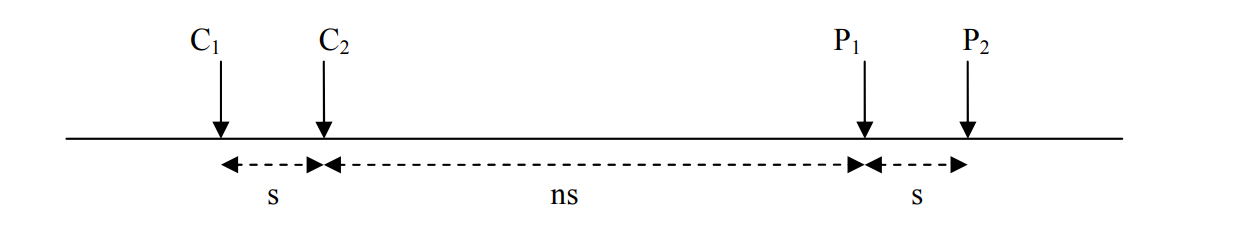
\includegraphics[width=0.8\textwidth]{figs/fig11.png}
    \caption{Image for questions 54,55}
    \label{fig:question54,55}
\end{figure}

\begin{enumerate}
\setcounter{enumi}{53}


\item The geometrical factor for the above axial dipole array is  
\begin{multicols}{4}
\begin{enumerate}
\item \(\pi n (n+1) s\)  
\item \(\pi n (n+2) s\)  
\item \(\pi (n+1)(n+2) s\)  
\item \(\pi n (n+1)(n+2) s\)  
\end{enumerate}
\end{multicols}

\item What is the apparent resistivity (in \(\Omega\)m) if 1.0 Amp current flowing between C1 and C2 produces 10 mV potential difference between P1 and P2 for \(s = 10\, \text{m}\) and \(n = 10\)? (Use \(\pi = 3.14\))  
\begin{multicols}{4}
\begin{enumerate}
\item 414.48  
\item 41.45  
\item 37.68  
\item 34.54  
\end{enumerate}
\end{multicols}

\end{enumerate}

\newpage
\section*{\textbf{General Aptitude (GA) Questions }}
\vspace{0.5cm}

\setcounter{enumi}{55}
\begin{enumerate}[resume]
\item Choose the most appropriate word or phrase from the options given below to complete the following sentence.  
\textbf{The environmentalists hope the lake }\underline{\hspace{2cm}} its pristine condition.  
\begin{enumerate}
\item in restoring  
\item in the restoration of  
\item to restore  
\item restoring  
\end{enumerate}

\item Choose the word from the options given below that is most nearly opposite in meaning to the given word: \textbf{Polemical}  
\begin{enumerate}
\item imitative  
\item conciliatory  
\item truthful  
\item ideological  
\end{enumerate}

\item Choose the most appropriate word from the options given below to complete the following sentence.  
\textbf{Despite the mixture's \underline{\hspace{1cm}} nature, we found that by lowering its temperature in the laboratory we could dramatically reduce its tendency to vaporize.  }
\begin{enumerate}
\item acerbic  
\item resilient  
\item volatile  
\item heterogeneous  
\end{enumerate}

\item If \(m\) students require a total of \(m\) pages of stationery in \(m\) days, then 100 students will require 100 pages of stationery in  
\begin{multicols}{4}
\begin{enumerate}
\item 100 days  
\item \(m/100\) days  
\item \(100/m\) days  
\item \(m\) days  
\end{enumerate}
\end{multicols}

\item Choose the most appropriate words from the options given below to complete the following sentence.  
\textbf{Because she had a reputation for \underline{\hspace{1cm}}, we were surprised and pleased when she greeted us so \underline{\hspace{1cm}}. } 
\begin{enumerate}
\item insolence ...... irately  
\item insouciance ......curtly  
\item graciousness ......amiably  
\item querulousness ...... affably  
\end{enumerate}

\item The number of solutions for the following system of inequalities is  
\[
x_1 \geq 0,\quad x_2 \geq 0,\quad x_1 + x_2 \leq 10,\quad 2x_1 + 2x_2 \geq 22
\]  
\begin{multicols}{4}
\begin{enumerate}
\item 0  
\item infinite  
\item 1  
\item 2  
\end{enumerate}
\end{multicols}

\item In a class of 300 students in an M.Tech programme, each student is required to take at least one subject from the following three: \\ 
M600: Advanced Engineering Mathematics  \\
C600: Computational Methods for Engineers \\ 
E600: Experimental Techniques for Engineers \\ 
The registration data for the M.Tech class shows that 100 students have taken M600, 200 students have taken C600, and 60 students have taken E600. What is the maximum possible number of students in the class who have taken all the above three subjects? 
\begin{multicols}{4}
\begin{enumerate}
\item 20  
\item 30  
\item 40  
\item 50  
\end{enumerate}
\end{multicols}

\item Three sisters (R, S, and T) received a total of 24 toys during Christmas. The toys were initially divided among them in a certain proportion.n. Subsequently, R gave some toys to S which doubled the share of S. Then S in turn gave some of her toys to T, which doubled T\'s share. Next, some of T\'s toys were given to R, which doubled the number of toys that R currently had. As a result of all such exchanges, the three sisters were left with equal number of toys. How many toys did R have
originally? 
\begin{multicols}{4}
\begin{enumerate}
\item 8  
\item 9  
\item 11  
\item 12  
\end{enumerate}
\end{multicols}

\item The quality of services delivered by a company consists of six factors as shown below in the radar diagram. The dots in the figure indicate the score for each factor on a scale of 0 to 10. The standardized coefficient for each factor is given in the parentheses. The contribution of each factor to the overall service quality is directly proportional to the factor score and its standardized coefficient.  

\begin{figure}[H]
    \centering
    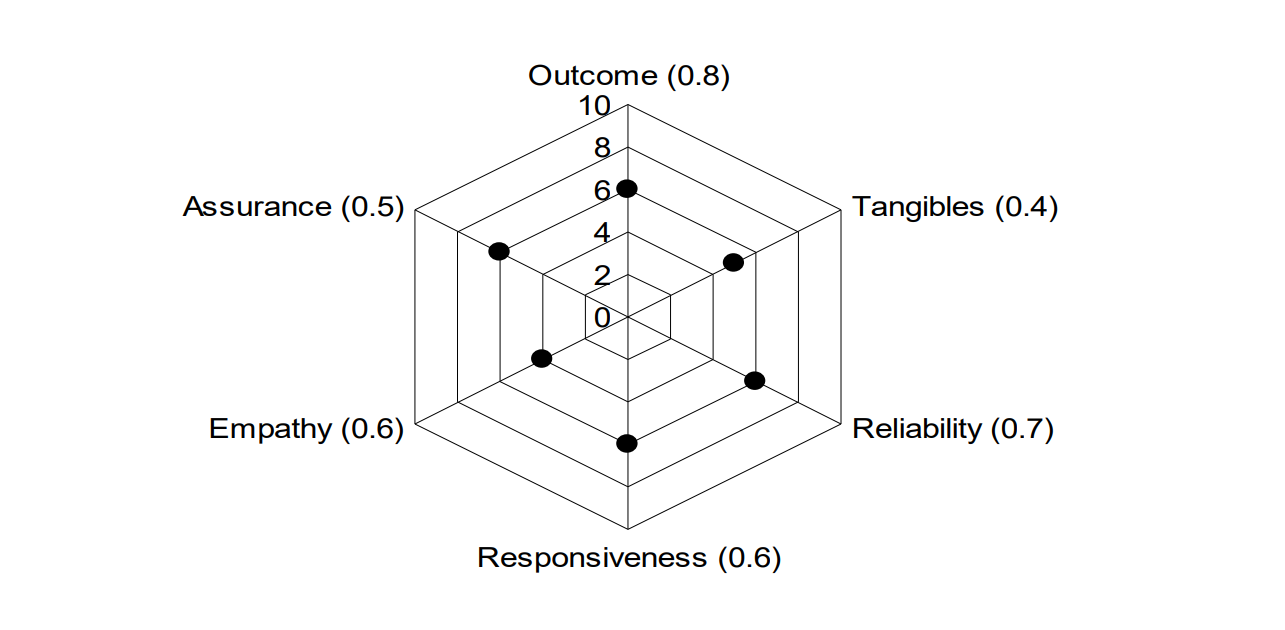
\includegraphics[width=0.8\textwidth]{figs/fig12.png}
    \caption{Image for questions 64}
    \label{fig:question64}
\end{figure}
Which factor contributes the least?  
\begin{multicols}{4}
\begin{enumerate}
\item 10%  
\item 20%  
\item 24%  
\item 40%  
\end{enumerate}
\end{multicols}


\item \textbf{In order to develop to full potential, a baby needs to be physically able to respond to the environment.}  
It can be inferred from the passage that  
\begin{enumerate}
\item Full physical potential is needed in order for a baby to be able to respond to the environment.  
\item It is necessary for a baby to be able to physically respond to the environment for it to develop its full potential.  
\item Response to the environment of physically able babies needs to be developed to its full potential.  
\item A physically able baby needs to develop its full potential in order to respond to its environment.  
\end{enumerate}

\end{enumerate}


\end{document}